\section{Evaluation}

\textbf{Environment and Workloads:}




\subsection{SciSpot Performance and Cost}

\begin{figure}
  \centering
  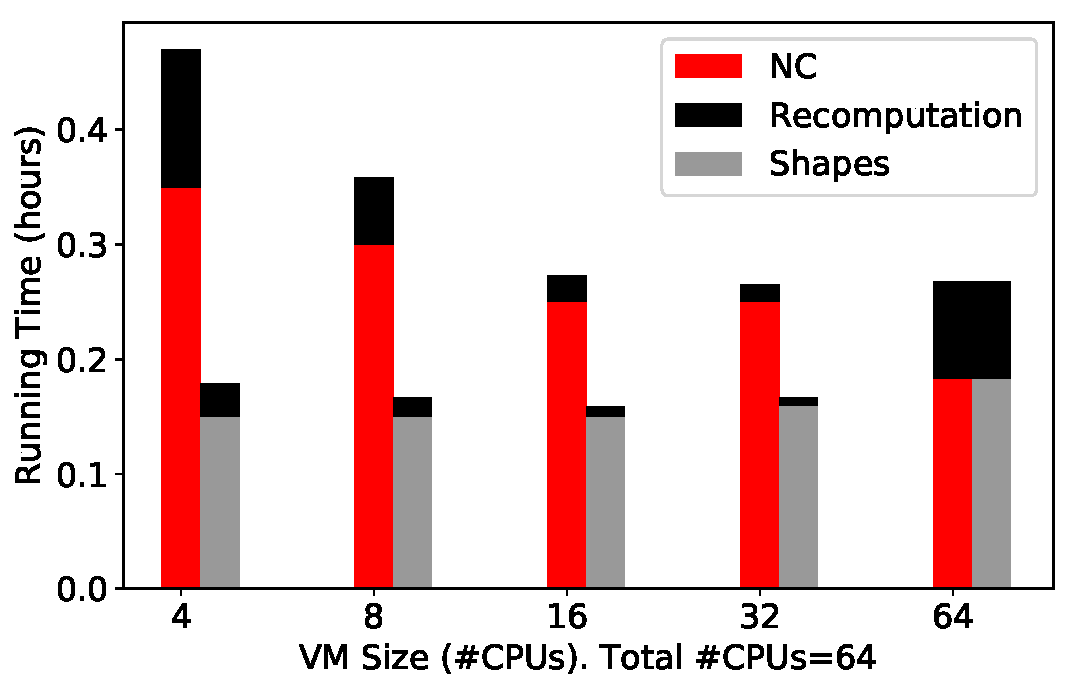
\includegraphics[width=0.4\textwidth]{../graphs/cost-bars.pdf}
  \caption{Running times of applications on different servers}
  \label{fig:runtimes-bar}
\end{figure}

\emph{Result: Running time is cluster configuration dependent, and increase in running time due to recomputation is small and less thna 5\%.}



\begin{figure}
  \centering
  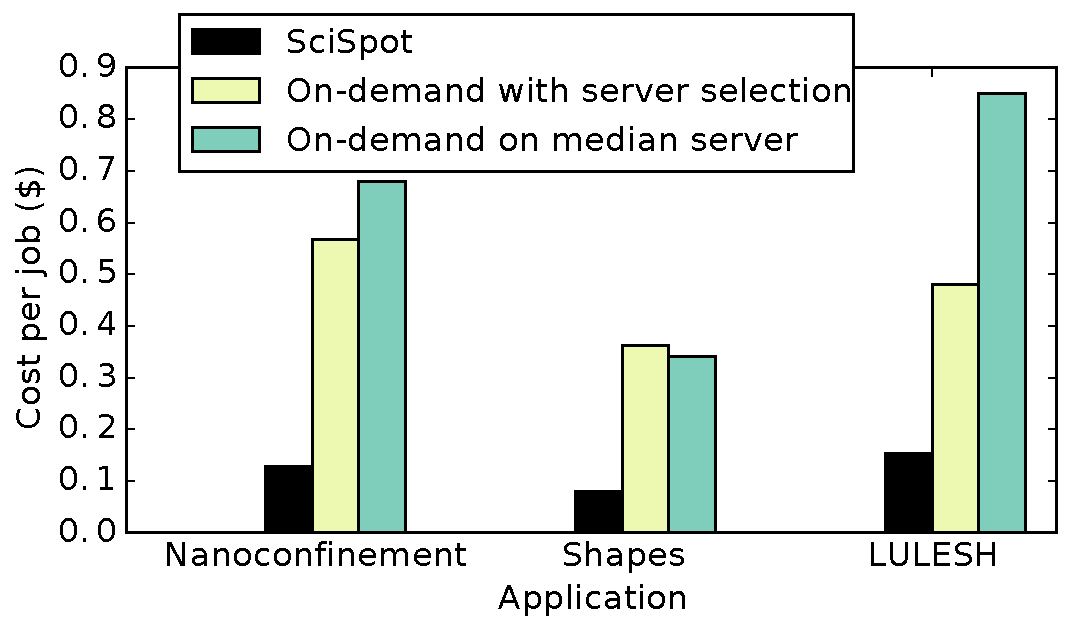
\includegraphics[width=0.4\textwidth]{../graphs/cost-only-bar.pdf}
  \caption{Cost of different configurations}
  \label{fig:cost-only-bar}
\end{figure}

\emph{Result: SciSpot reduces computing costs by up to 5x and 7x compared to on-demand cloud servers.}

\begin{figure}
  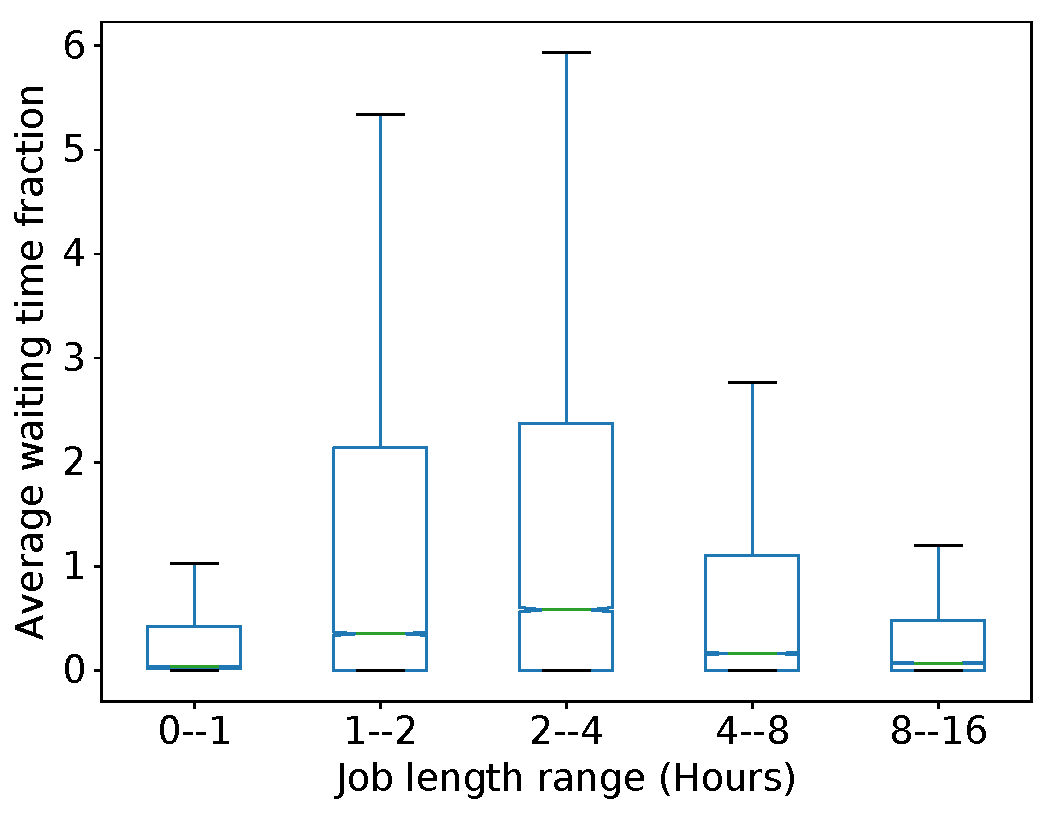
\includegraphics[width=0.4\textwidth]{../graphs/waiting_time_buckets.pdf}
  \caption{Waiting time fraction of jobs of different lengths varies.}
  \label{fig:hpc-wait-buckets}  
\end{figure}



\subsection{Total cost vs. running time graphs}

\begin{figure}
  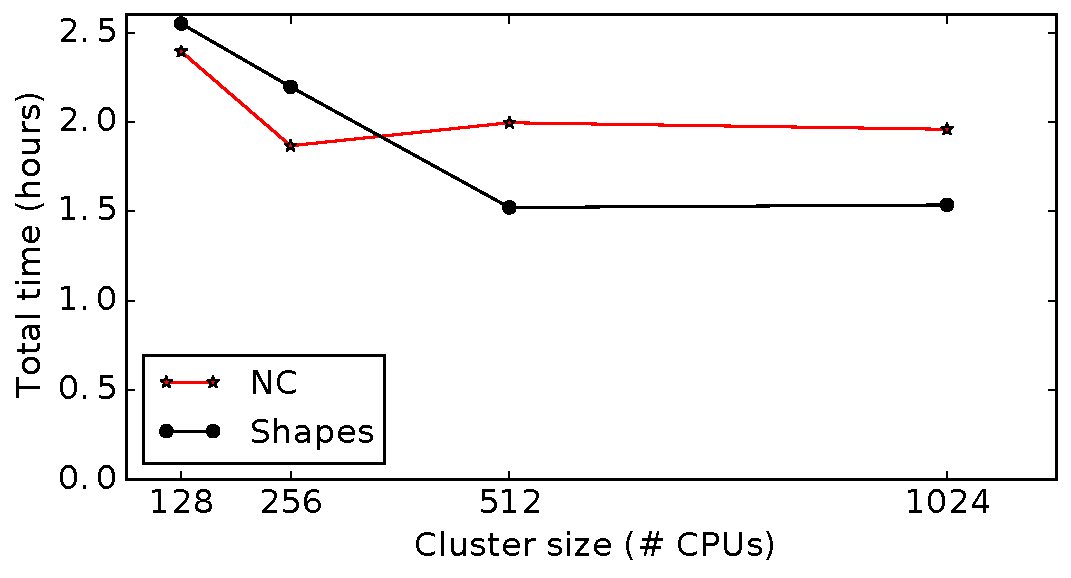
\includegraphics[width=0.2\textwidth]{../graphs/vm-per-job-scaling.pdf}
  \caption{SciSpot scaling as the VMs per jobs increases}
  \label{fig:vm-per-job-scaling}
\end{figure}

Figure~\ref{fig:vm-per-job-scaling} shows the total bag of job execution times for 32 jobs with 4 jobs running in parallel.
32 CPU VM's were used, and thus the total number of CPUs = 32*jobs-per-VM. Max CPU's used was 512 


\begin{figure}
  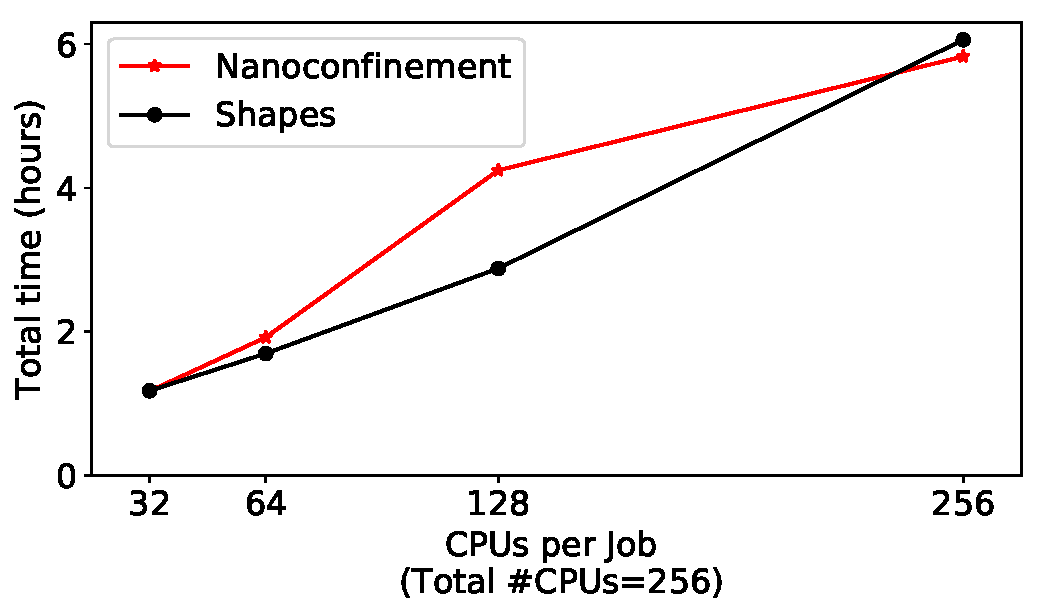
\includegraphics[width=0.2\textwidth]{../graphs/par-scaling.pdf}
  \caption{Job running times as the CPU's per job increases}
  \label{fig:par-scaling}
\end{figure}

Figure~\ref{fig:par-scaling} shows the running time when the total cluster size is fixed, but the number of parallel jobs and hence the number of CPUs per job changes. 



\subsection{Comparison with HPC Clusters}


% \begin{figure}
%   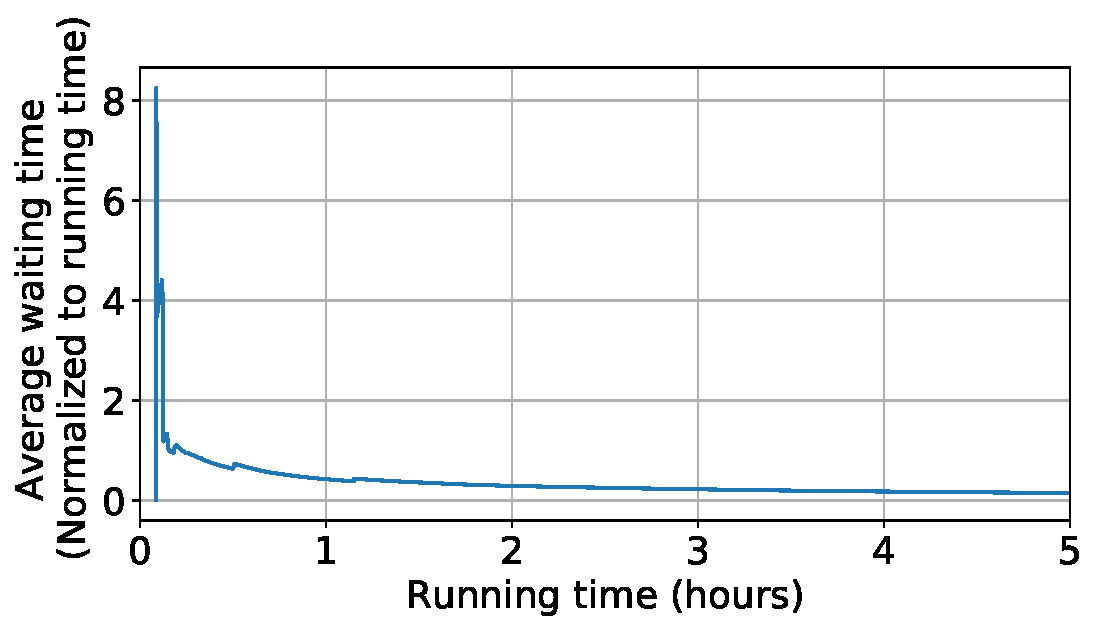
\includegraphics[width=0.4\textwidth]{../data/waiting_cumul.pdf}
%   \caption{The average waiting time (normalized to running time) of jobs of different length.}
%   \label{fig:hpc-wait-cdf}
% \end{figure}



%%% Local Variables:
%%% mode: latex
%%% TeX-master: "paper"
%%% End:
